Elementarteilchen sind die kleinsten bekannten Elemente, die sich nicht weiter zerteilen lassen.
Diese Teilchen werden in die Gruppen der Quarks und Leptonen unterteilt.
Diese unterscheiden sich in der Art ihrer Wechselwirkung.
Die Leptonen, die eine schwache Wechselwirkung besitzen, werden weiter in drei Generationen unterteilt, welche sich wiederum in Masse und Stabilität unterteilen.
Die Ladung bleibt hingegen konnstant bei einer Elementarladung.
Das hat zur Folge, dass Leptonen neben der schwachen Wechselwirkung ebenso einer elektromagnetischen Wechselwirkung unterliegen.
In der Tabelle \ref{tab:gen} können die generationszugehörigen Elementarteilchen eingesehen werden.
Das Elektron, welches der ersten Generation angehört, besitzt die geringste Masse und ist stabil.
Mit steigender Generation steigt die Masse an und die Stabilität nimmt ab.
Das Myon besitzt dementsprechend schon eine endliche Lebensdauer, nach der es zerfallen kann.
\begin{table}[h!]
  \centering
  \caption{Liste der Leptonen \cite{1}}
  \label{tab:gen}
  \begin{tabular}{l r r l l}
    \toprule
%    \multicolumn{3}{c}{$f_{\text{1, theo}}=\SI{0.1}{m}$} & \multicolumn{3}{c}{$f_{\text{2, theo}}=\SI{0.05}{m}$}\\
      Generation & Teilchen & Antiteilchen  \\
      \midrule
      1.& Elektron $e^{-}$                   &   Positron $e^{+}$    \\
      2.& Myon   $\mu^{-}$                   &          $\mu^{+}$    \\
      3.& Tauon $\tau^{-}$                   &         $\tau^{+}$    \\
      \midrule
        & Elektron-Neutrino $\nu_{\text{e}}$ & $\overline{\nu}_{\text{e}}$\\
        & Myon-Neutrino     $\nu_{\mu}$      & $\overline{\nu}_{\mu}$     \\
        & Tauon-Neutrino    $\nu_{\tau}$     & $\overline{\nu}_{\tau}$    \\
    \bottomrule
  \end{tabular}
\end{table}
%\begin{figure}[h!]
%  \centering
%  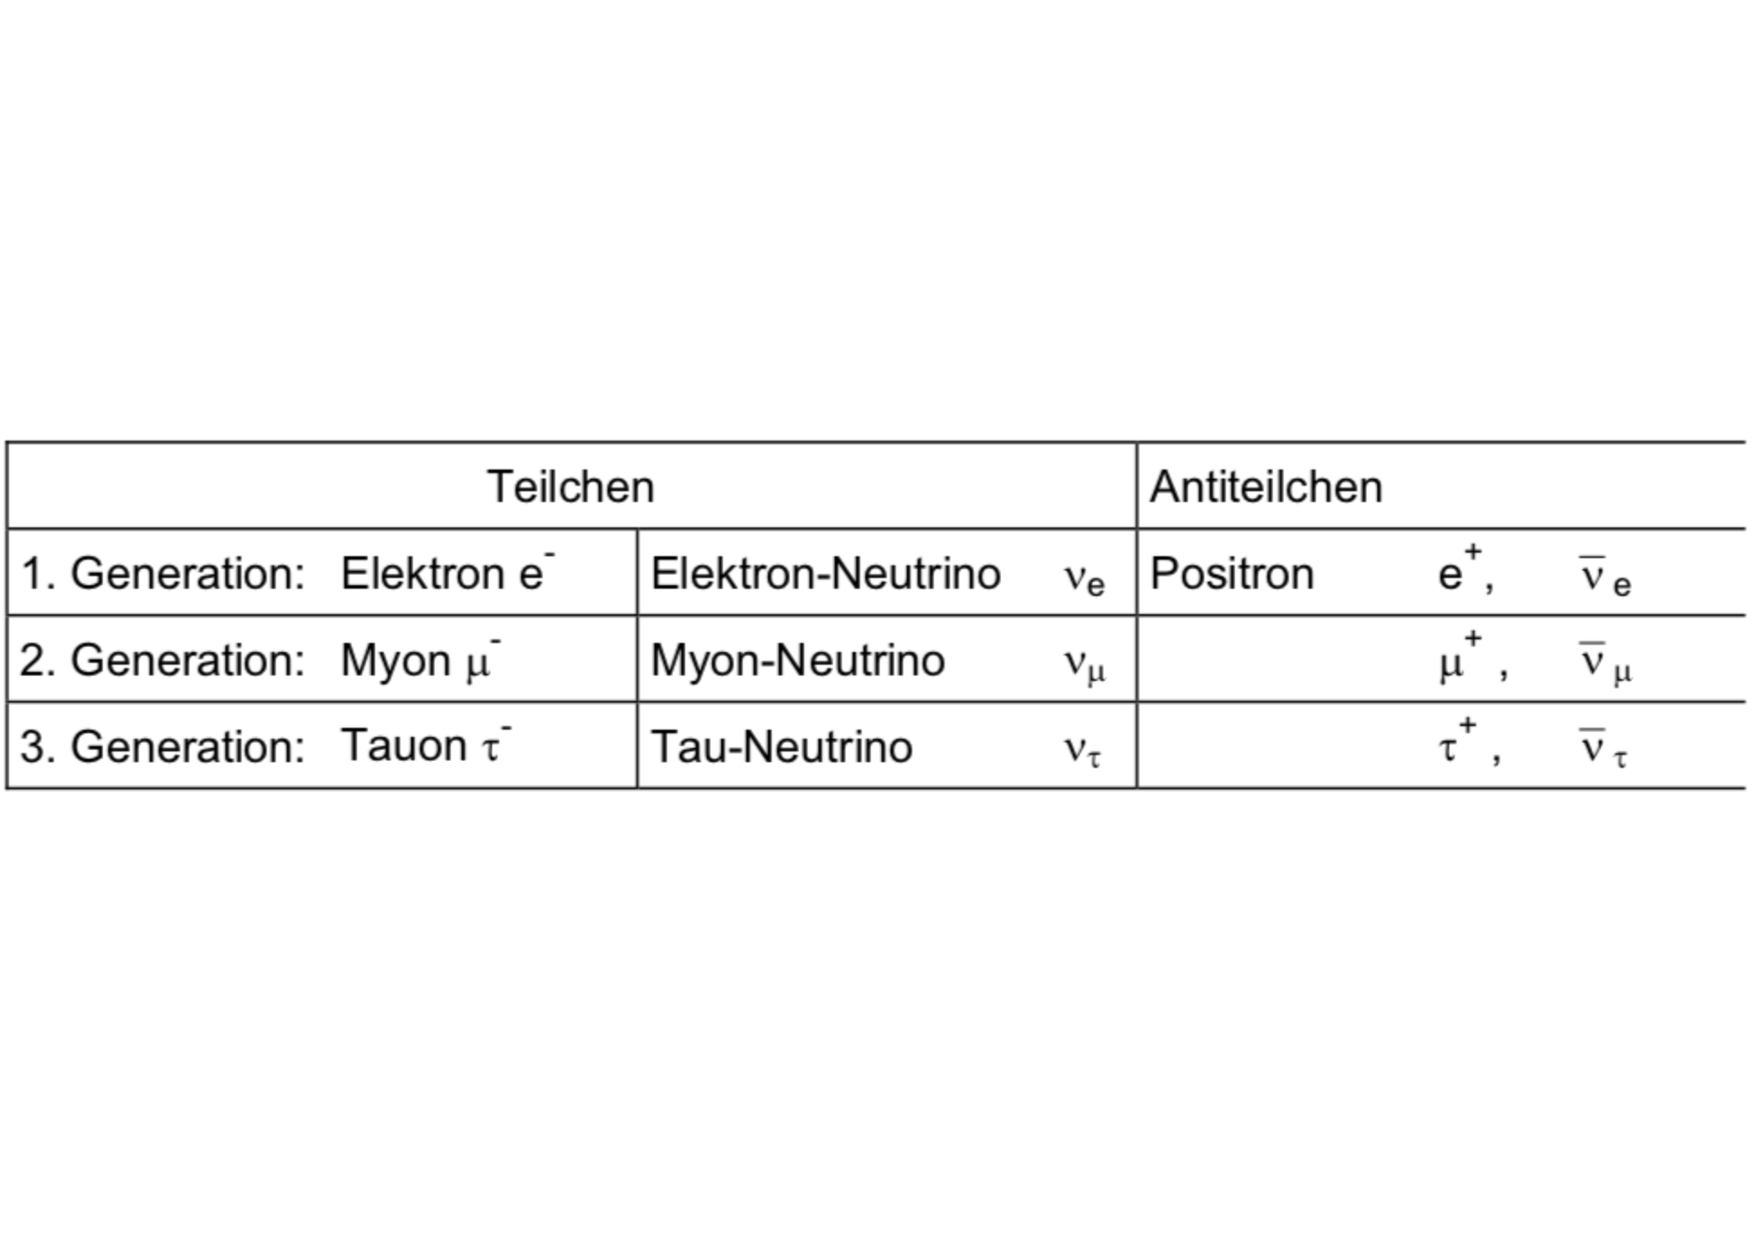
\includegraphics[width=\textwidth]{tableptonen.pdf}
%  \caption{Liste der Leptonen \cite{1}}
%  \label{tab:gen}
%\end{figure}
\FloatBarrier

Mit Hilfe der ebenfalls in der Tabelle \ref{tab:gen} aufgeführten spezifischen Neutrinos und Antiteilchen
werden die Erhaltungsgrößen Energie, Impuls und Drehimpuls bei einem Zerfall von Leptonen nicht verletzt.
Daraus ergibt sich für den Zerfall von Myonen:
\begin{align}
  \mu^{-}\rightarrow e^-+\overline{\nu}_\text{e}+\nu_{\mu}.
  \label{eqn:mu-}
\end{align}
Das Antimyon zerfällt dementsprechend zu:
\begin{align}
  \mu^{+}\rightarrow e^++\nu_\text{e}+\overline{\nu}_{\mu}.
  \label{eqn:mu+}
\end{align}

Der Zerfall ist ein statistischer Prozess. Das heißt, dass sich die individuellen Lebensdauern stark unterscheiden können.
Für einen infinitesimalen Bereich kann die Wahrscheinlichkeit dW als propotional zu der Beobachtungszeit betrachtet werden.
\begin{align}
  \text{dW}=\lambda \text{dt}
  \label{eqn:W}
\end{align}
Die Konstante $\lambda$ wird als Zerfallskonstante beschrieben.
Der Gleichung \ref{eqn:W} ist zu entnehmen, dass der Zerfallsprozess unabhängig von t ist.
Daraus lässt sich folgern, dass Elementarteilchen keinem Alterungsprozess unterliegen.

Durch das Erweitern auf N Teilchen lässt sich die Gleichung intergrieren und für den Zeitraum t bis t+dt betrachten.
\begin{align}
  \frac{\text{dN(t)}}{\text{N}_0}=\lambda e^{-\lambda \text{t}} \text{dt}
  \label{eqn:e}
\end{align}



$\text{N}_0$ beschreibt die Gesamtzahl der betrachteten Teilchen.
Anhand der Gleichung \ref{eqn:e} wird deutlich, dass es sich um einen Exponential-Verteilung handelt.
Beschreibt man die Lebensdauer $\tau$ einer speziellen Teilchenart ergibt sich:
\begin{align*}
  \tau=\int_{-\infty}^{\infty}\lambda \text{t} e^{-\lambda \text{t}}\text{dt}=\frac{1}{\lambda}.
\end{align*}

Mit Hilfe einer Stichprobe, das heißt mit endlich vielen Messergebnissen n, lässt sich eine Abschätzung der Lebensdauer vornehmen.
Die durch die Stichprobe ermittelte Lebensdauer $\overline{\text{t}}$ sollte möglichst genau an den tatsächlichen Wert der Lebensdauer $\tau$ herankommen.
Dies erreicht man mit dem arithmetische Mittel aus n Lebensdauern t.
\begin{align*}
  \overline{\text{t}}:=\frac{1}{\text{n}}\sum_{\text{j}=1}^\text{n}\text{t}_\text{j}
\end{align*}
Es gilt:
\begin{align*}
  \text{E}\overline{\text{t}}=\tau.
\end{align*}
Der Fehler der Abschätzung ist gegeben durch die Varianz $\sigma$
\begin{align*}
  \sigma^2:=\int_{-\infty}^{\infty}\text{f(t)}(\text{t}-\tau)^2\text{dt}.
\end{align*}


Treffen energiereiche Photonen der kosmischen Höhenstrahlung auf Atomkerne der Luftmoleküle enstehen durch Wechselwirkungen
Pionen.
Diese zerfallen wiederum wegen ihrer kurzlebigkeit in der Atmosphäre zu Myonen.
\begin{align*}
  \pi^+ \rightarrow \mu^++\nu_\mu\\
  \pi^- \rightarrow \mu^-+\overline{\nu}_\mu
\end{align*}
Die Myonen bewegen sich mit annähernd Lichtgeschwindigkeit auf die Erde zu.
